\documentclass[a4paper,12pt]{article}
\usepackage[a4paper, margin=2.5cm, top=4cm]{geometry}
\usepackage{mathtools,amssymb,graphicx,float,caption,subcaption}
\usepackage[utf8]{inputenc}
\usepackage{biblatex}
\addbibresource{progress.bib}

\RequirePackage[T1]{fontenc}
\RequirePackage{lmodern}
\renewcommand\familydefault{\sfdefault}
% gives double-spacing
\linespread{1.6}


\title{Progress report}
\author{Alvin Jonel De la Cruz Guerrero - 20492499}
\date{1 June 2023}

\begin{document}
  \maketitle

  \section{Project Overview}

  My dissertation project is about Partial Differential Equations PDEs: Modelling and 
  Computation in Finance. Specifically, I am exploring how to price American options by 
  solving the system of PDE resulting from applying to black-schole-merton model to hedge
  the risk of the option. 
  
  \subsection{Background}
  An American option is a contract that gives the holder the right to buy, or 
  sell an underly stock $S$ at strike price $K$ at any point in time between the
  start ($t=0$) and expiration date ($t=T$) of the contract inclusively. At any 
  point in time $t \in [0, T]$, the 
  payoff function of an american call/put option can be defined as deterministc
  of the price at that time $S = S(t)$:

  \begin{equation}
    \begin{aligned}
    C(S) = \max(S - K, 0) & \quad \text{call option} \\
    P(S) = \max(K - S, 0) & \quad \text{put option}
    \end{aligned}
  \end{equation}

  Assuming that stock does not have dividends, pricing an American option 
  is similar to price an European option. Therefore, we focus on the pricing 
  American put options. The problem of pricing of American put options could be 
  reformulated as a free boundary. For the free boundary formulation, we are task to
  to find the value of the option $V(S, t)$ at time 0 while at same time finding 
  the optimal exercise price $\bar{S}(t)$, the exercise region 
  $\mathcal{C} := \{(S,t): S > \bar{S}(t)\}$, and the optimal 
  exercise boundary $\partial\mathcal{C} := \{(S,t): S = \bar{S}(t) \}$.

  \begin{figure}[H]
    \centering
    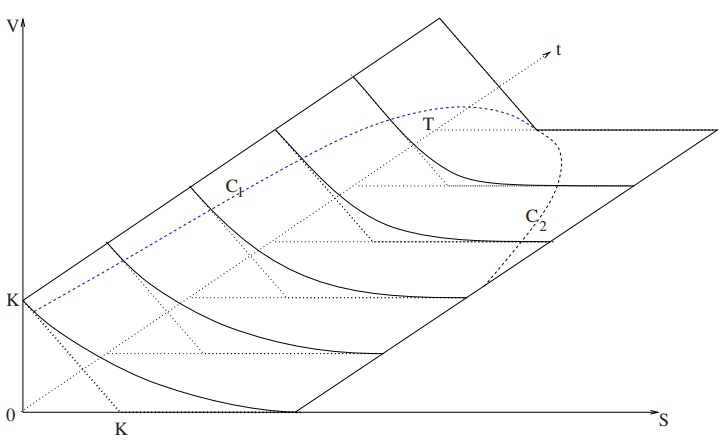
\includegraphics[scale=0.7]{progress_report/American_put_option.png}
    \caption{Value surface of an American option by Seidel\cite{seydel_2009}.}
    \label{fig:value_surface}
  \end{figure}

  The problem stated is described by the well known system of equation:

  \begin{equation}
    \begin{aligned}
      & \frac{\partial V}{\partial t} + \frac{1}{2}\sigma^2 S^2 \frac{\partial^2 V}{\partial S^2} + rS \frac{\partial V}{\partial S} - rV = 0 & \quad \text{for $S > \bar{S}(t)$ and $0 \leq t < T$} \\
      & V(T, S) = \max(K - S, 0) & \text{for $S \geq 0$} \\
      & \frac{\partial V}{\partial S}(t, \bar{S}(t)) = -1 \\
      & V(t, \bar{S}(t)) = K - \bar{S}(t) \\
      & \lim_{S \rightarrow \infty} V(t, \bar{S}(t)) = 0 \\
      & \bar{S}(T) = K \\
      & V(t, S) = K - S & \text{for $0 \leq S < \bar{S}(t)$} \\
    \end{aligned}   
    \label{eq:section_1:free_boundary_problem}
  \end{equation}

  For the given parameters $\sigma$ (price volatility) 
  and $r$ (risk-free interest rate).
  
  \section{Progress}

  In the week from the 12-18 of June, I read some of the materials provided to me, specifically, 
  the chapters 1-4 \cite*{hilber_reichmann_schwab_winter_2013}; section 1-3 of \cite*{nielsen_2001};.

  In the week from the 19-26 of June, I used the tranformation 
  
  \begin{equation}
    x = \frac{S(t)}{\bar{S}(t)}
    \label{eq:section_2:nielsen_tranformation}
  \end{equation}

  proposed by Nielsen \cite*{nielsen_2001}, to fix the free boundary in equation 
  (\ref{eq:section_1:free_boundary_problem}). Therefore, the value function
  depends on $x \in [0, \infty]$ that is fixed in time.

  \begin{equation}
    v(t, x) = V(t, x\bar{S}(t))
  \end{equation}

  Using (\ref{eq:section_2:nielsen_tranformation}) in (\ref{eq:section_1:free_boundary_problem}), 
  the system of equation (\ref{eq:section_1:free_boundary_problem}) is 
  reformulated as a system of non-linear PDEs: 

  \begin{equation}
    \begin{aligned}
      & \frac{\partial v}{\partial t} + \frac{1}{2}\sigma^2 x^2 \frac{\partial^2 v}{\partial x^2} + x\bigg(r - \frac{\bar{S}'(t)}{\bar{S}'(t)}\bigg)\frac{\partial v}{\partial x} - rv = 0 & \quad \text{for $x > 1$ and $0 \leq t < T$} \\
      & v(T, x) = 0 & \text{for $x \geq 1$} \\
      & \frac{\partial v}{\partial x}(t, 1) = -S(t) \\
      & v(t, 1) = K - \bar{S}(t) \\
      & \lim_{S \rightarrow \infty} v(t, x) = 0 \\
      & \bar{S}(T) = K
    \end{aligned}   
    \label{eq:section_2:nielsen_pde_system}
  \end{equation}

  Then I proceeded to solve the system in (4) by applying both the explicit and implicit finite difference schemes. 
  The code was written in python and to test the implementation, I used the same parameters listed in Nielsen \cite*{nielsen_2001}

  \begin{align*}
    r = 0.1 \\
    \sigma = 0.2 \\
    K = 1 \\
    T = 1 \\
    x_{\infty} = 2 \\
  \end{align*}

  using a grid resolution of $\Delta t = \Delta x = 0.0001$ for the explicit scheme, and
  $\Delta x = 5.0 \time 10^{-6}$ and $\Delta x = 0.001$. Below, there are the produced by
  my implementation of both scheme in python. As you can see both plots looks quite similar 
  to figure \eqref{fig:value_surface} where the solid orange line is the vale $V(S, t)$ of the option a time 0, the solid blue
  is the payoff function of the american put option and the dashed blue line is the optimal
  exercise price $\bar{S}(t)$ at time 0.

  \begin{figure}[H]
    \centering
    \begin{subfigure}[b]{0.5\textwidth}
        \centering
        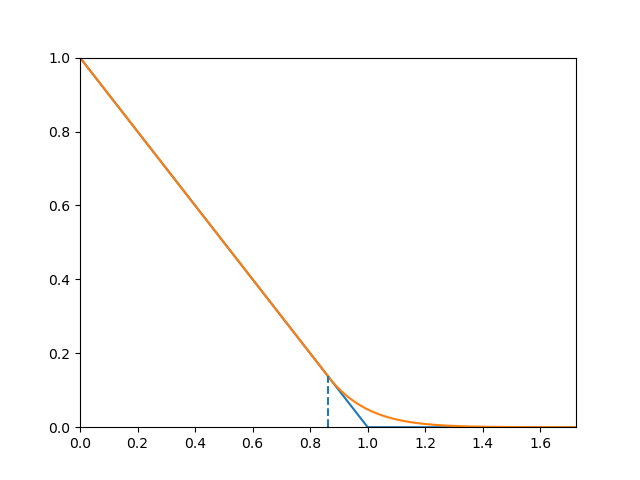
\includegraphics[width=\textwidth]{progress_report/Front_fixing_explicit_FD.png}
        \caption{$\bar{S}(0) = 8.6232 \times 10^{-1}$}
        \label{fig:y equals }
    \end{subfigure}
    \hspace{-1cm}
    % \hfill
    \begin{subfigure}[b]{0.5\textwidth}
        \centering
        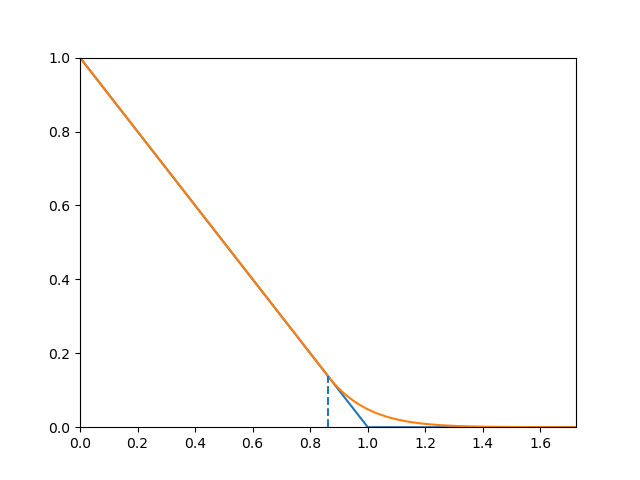
\includegraphics[width=\textwidth]{progress_report/Front_fixing_implicit_FD.png}
        \caption{$\bar{S}(0) = 8.6178 \times 10^{-1}$}
        \label{fig:three sin x}
    \end{subfigure} 
    \caption{American put option value at time 0. The left and right plots are 
    from apply an explicit and implicit scheme respectevely.}
    \label{fig:explicit_implicit_fd}
  \end{figure}

  \section{Future work}

  Another reformulation of the pricing problem or an American put option is the 
  linear complmentary problem. My plan for the week from 3-9 of July is to solve
  the Linear Complementary problem for an american option using the PSOR method. 
  
  During the week 10-17 of July, I will explore directions my dissertation could take. 
  The original plan is to do a comparative numerical analysis of each the methods. 
  However, I would like to explore other possibilities. For instance, 
  pricing american call options with dividends, solving the problem of pricing an 
  american put option using jump diffusion models instead of the black scholes 
  model by solving a Partial Integro-Differential equation, or pricing american swaptions
  using numerical PDEs.
  
  \medskip

  \printbibliography
  
\end{document}

